\documentclass[a4paper,12pt]{article}

\usepackage{graphicx}
\usepackage{amsmath}
\usepackage{tkz-euclide}

\begin{document}
\title{Assignment 7}
\author{Junaid Ahmad Bhat}
\date{January 25, 2021}
\maketitle
\section*{{\small Question}}
Draw a circle with centre B and radius 6. If
C be a point 10 units away from its centre,
construct the pair of tangents AC and CD to
the circle.
\section*{{\small Solution}}

\begin{center}
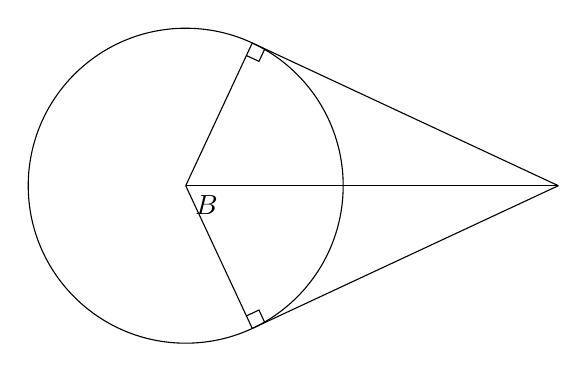
\begin{tikzpicture}
\xdef\r{2}
\xdef\ang{65}
\xdef\side{5pt}
\coordinate (B) at (0,0)node[below right]{$B$};
\draw (B) circle[radius=\r];
\draw (B)--([shift=(\ang:\r)]B) coordinate(b);
\draw (b)--({\r*sec(\ang)},0) coordinate(A) node[midway, rotate={-\ang-90}]{}; 
\draw (B)--([shift=(-\ang:\r)]B) coordinate(C); 
\draw (C)--({\r*sec(-\ang)},0) coordinate(D) node[midway, rotate={-\ang-90}]{};
\draw ($(b)!\side!(B)$) -- ($($(b)!\side!(B)$)!\side!90:(B)$) -- ($(b)!\side!(A)$);
\draw ($(C)!\side!(A)$) -- ($($(C)!\side!(A)$)!\side!90:(A)$) -- ($(C)!\side!(B)$);
\draw (B)--(D) node[midway]{};
\end{tikzpicture}
\end{center}
\hspace*{4cm}Rough sketch with O as origin\\

\textbf{TO draw the circle and the tangents to the given circle with
\hspace*{0.5cm} radius = 6,we need to find the coordinates of points of\\ \hspace*{0.5cm}intersection of tangents}\\
 
Procedure is given below:\\

1.First, draw a given circle with B(0,0) as centre and radius = 6. \\

2.Now,We have to draw a circle with B and given external point C as diameter.\\

3.Coordinates of C are(10,0) as it is 10 units from centre of given circle\\

4.Therefore,center of circle mentioned in step 2 is S(5,0) and radius = 5 ,draw it.\\

5.Now,we have two known circles with known centres and known radius.\\

6.Writing equations of above two circles in standard form\\

\textbf{C1:x$^2$ + y$^2$ = 36 }   \hspace*{3cm}(centre B(0,0),radius = 6)\hspace*{1cm}(1)\\

\textbf{C2:(x-5)$^2$ + y$^2$ = 25}  \hspace*{2.5cm}(centre S(5,0),radius = 5)\hspace*{1cm}(2)\\

7.Let's find out the points of intersection of two circles\\
 
 \begin{center}
 Subtracting the eqn (2) from eqn (1),we get\\
  x=3.6 \hspace*{10.5cm}(3)\\
 Subtstuting the value of x from eqn (3) into eqn (1),we get\\
  y=4.8,-4.8 \hspace*{10cm}(4)\\        
 \end{center}

8.Therefore from eqn(3) and eqn(4),we get the coordinates of A and D   \hspace*{1cm} respectively\\

9.Finally,we have Coordinates of A(3.6,4.8),D(3.6,-4.8) and C(10,0).\\

10.Below figure is the required construction.
\begin{figure}[h]
\centering
\includegraphics[width=0.6\textwidth]{A7}
\caption{Figure using python}
\end{figure}


\end{document}
